\section{Supporting material: an audit with positive controls}
\label{app:snapping}
% src: docs/findings/snapping-audit.md (per-session table, reading, flagged list, skipped
%      sessions) and docs/findings/snapping-audit.png; docs/STATUS.md (P0 row) for the
%      archive size. Ranges below are min / median / max over the 85 session rows of the
%      table in docs/findings/snapping-audit.md, computed from that table.
% Lockbox note: this audit registers public F1 telemetry against real circuit geometry. It
% computes no agent return and no optimum on any circuit, which the plan allows.

This appendix is not used by any claim in the paper. It is included because it applies the
same discipline as the audit, a measurement validated with planted signals before it is
trusted, to the public data that a companion analysis of human drivers depends on, and
because its result fixes what that analysis can and cannot claim.

\paragraph{Question} Public Formula One timing data include car positions at about
3.7\,Hz. Do these positions carry each driver's racing line, or are they projected onto a
single track model? It has been stated informally that they carry no lateral line; we are
not aware of a quantitative audit.
% src: docs/plan/novelty-and-outputs.md (C6, FastF1 Discussion #116, OpenF1 docs)
\VERIFY{the claim of no prior quantitative audit rests on the plan's prior-art search}

\paragraph{Method} For every qualifying session, each flying lap's position samples are
compared with a cubic-spline curve through the pole lap. Two tests are run: the distance
of every sample from that curve, and whether a driver's \emph{signed} lateral offset is
consistent across their own laps at each 50\,m station (one-way ANOVA and the intraclass
correlation, ICC). Three positive controls check that the test can see a line if one is
there: pit-lane samples, which are metres from the racing line; whole laps shifted by known
offsets of 1--3\,m; and a planted 0.5\,m line for one driver.
% src: docs/findings/snapping-audit.md (opening paragraph)
The data are 85 sessions from 2023--26 with \num{8183} flying laps (OpenF1, CC BY-NC-SA
4.0; aggregate statistics only), drawn from an archive of 111 sessions whose 5,196 files
were all checksum-verified.
% src: docs/findings/snapping-audit.md (85 rows; laps column summed); docs/STATUS.md (P0 row)

\paragraph{Result} Every session looks the same. Samples sit a median 9.4--13.3\,cm from
the pole lap's curve (median over sessions 11.3\,cm), while pit-lane samples sit metres
away (95th percentile 7.9\,m or more in every session), so the feed can represent
off-line positions. Injected 2\,m offsets are recovered as 1.99--2.02\,m. Drivers'
offsets are not consistent: the median per-session driver ICC is 0.006 (range $-0.019$ to
$+0.068$). The planted 0.5\,m line, by contrast, reaches an ICC of 0.57--0.88 and is
detected at 88--100\% of stations (median 98\%).
% src: docs/findings/snapping-audit.md (columns "Median dist.", "Pit-lane p95", "Injected 2 m ->",
%      "Driver ICC", "Planted ICC", "Planted detected"; min / median / max over 85 rows)
A median of 3.5\% of stations (range 0--12.1\%) are individually significant at
$p < 0.01$. That is above the nominal 1\% but far below the planted line's rate; the source
report attributes the excess to centimetre-scale per-car artefacts such as antenna
position or latency, an explanation we have not tested.
% src: docs/findings/snapping-audit.md (column "Stations p<0.01"; "Flagged for follow-up" paragraph)
Twenty-two sessions are flagged as open items (more than 5\% of stations significant, or
driver offsets above 20\,cm at the 95th percentile, the latter only for the two
Silverstone sessions at about 40\,cm); one car with a coordinate stream about 3\,m off
everywhere was excluded and reported, and two sessions were skipped.
% src: docs/findings/snapping-audit.md ("Flagged for follow-up" list: 22 entries; "Excluded
%      cars": 2023 Jeddah car 21; "Skipped sessions": 2)

\begin{figure}[h]
\centering
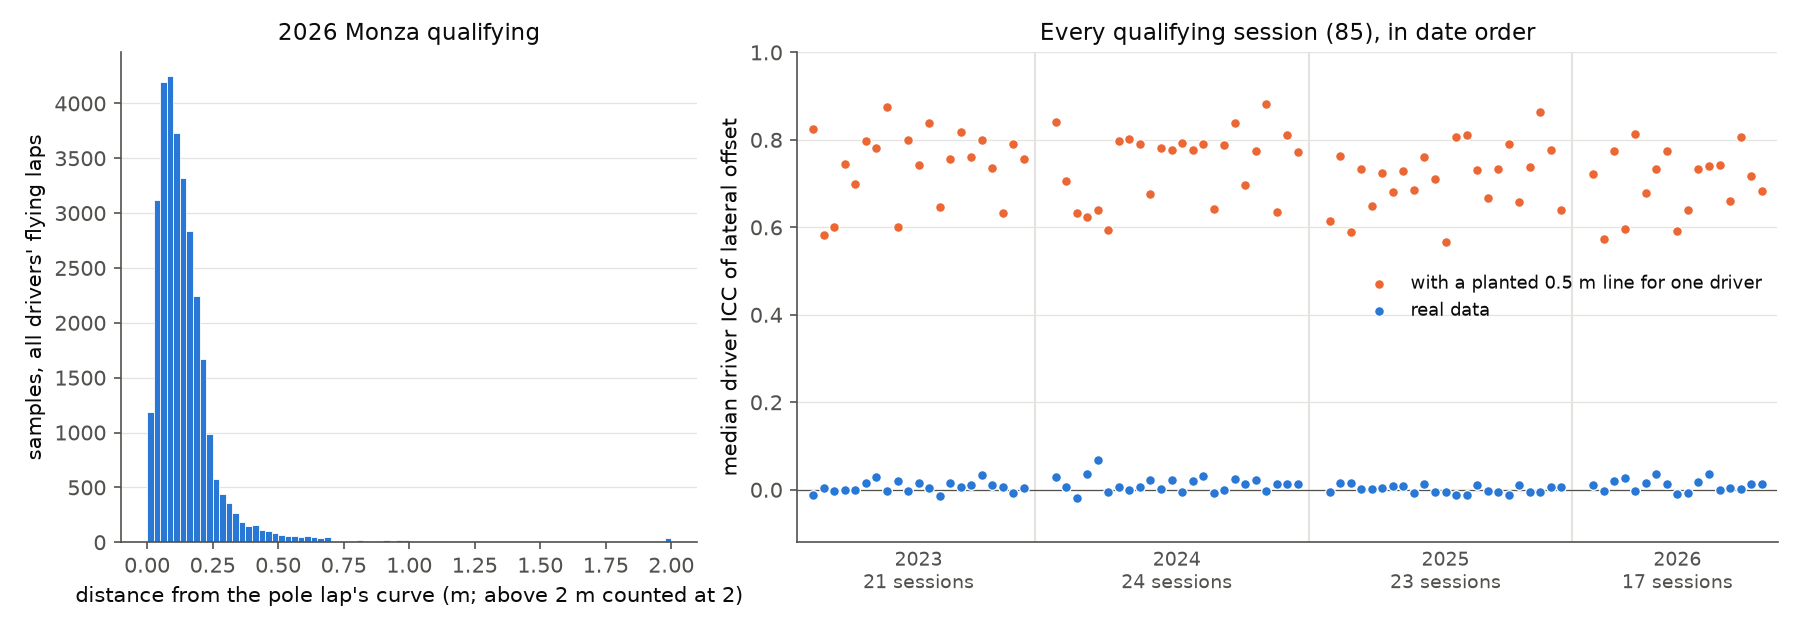
\includegraphics[width=\linewidth]{snapping-audit.png}
\caption{Left: distance of all drivers' flying-lap samples from the pole lap's curve in one
session. Right: median driver ICC of the signed lateral offset per session, for the real
data and with a planted 0.5\,m line. Reproduced from docs/findings/snapping-audit.png.}
\label{fig:snapping}
\end{figure}
\TODO{regenerate the right panel with legible session labels}

\paragraph{Consequence} The positions are projected onto one track model. Comparisons of
human drivers therefore use speed, throttle, brake and time as functions of distance,
never lateral lines. For this paper the lesson is methodological: a null result counts
only when the same pipeline demonstrably detects a planted signal of the size in question.
